% Inspired from
% https://github.com/andiac/gemini-cam
% a fork of https://github.com/anishathalye/gemini
% also refer to https://github.com/k4rtik/uchicago-poster

\documentclass[final]{beamer}

% ====================
% Packages
% ====================

\usepackage[T1]{fontenc}
\usepackage[utf8]{luainputenc}
\usepackage{lmodern}
\usepackage[orientation=portrait,size=a0,scale=1.0]{beamerposter}
\usetheme{gemini}
\usecolortheme{cnrs}
\usepackage{graphicx}
\usepackage{booktabs}
\usepackage{tikz}
\usepackage{pgfplots}
\pgfplotsset{compat=1.18}
\usepackage{anyfontsize}
\usepackage{xcolor}
\usepackage{dirtytalk}
\usepackage{wrapfig}
% \usepackage{hyperref}

\usepackage[
  backend=biber,
  style=numeric,
  sorting=ynt,
  url=false,
  doi=false,
  isbn=false,
]{biblatex}
\addbibresource{poster.bib}

\usepackage{unicode-math}
\setmathfont[Scale=MatchUppercase]{libertinusmath-regular.otf}

\usepackage[margin=10pt,
            % labelfont=bf,
            % labelsep=endash,
            format=plain,
]{caption}
\usepackage{amsmath,amssymb}
\usepackage{siunitx}
\usepackage{physics2}
\usephysicsmodule{ab} % automatic bracing

% macros for \vb, \va and \vu
\makeatletter
\newcommand\vb{\@ifstar\boldsymbol\mathbf}
\newcommand\va[1]{\@ifstar{\vec{#1}}{\vec{\mathrm{#1}}}}
\newcommand\vu[1]{%
\@ifstar{\hat{\boldsymbol{#1}}}{\hat{\mathbf{#1}}}}
\makeatother

\newcommand{\transpose}[1]{\ensuremath{#1^{\mathsf T}}}

% ====================
% Lengths
% ====================

% If you have N columns, choose \sepwidth and \colwidth such that
% (N+1)*\sepwidth + N*\colwidth = \paperwidth
\newlength{\sepwidth}
\newlength{\colwidth}
\setlength{\sepwidth}{0.025\paperwidth}
\setlength{\colwidth}{0.45\paperwidth}

\newcommand{\separatorcolumn}{\begin{column}{\sepwidth}\end{column}}

% ====================
% Title
% ====================

\title{Map-making strategies for next generation CMB polarization experiments}

\author{Simon Biquard \inst{1} \and Radek Stompor \inst{2, 1} \and Josquin Errard \inst{1}}

\institute[shortinst]{\inst{1} AstroParticule et Cosmologie, Paris, France \samelineand \inst{2} Centre Pierre Binétruy, Berkeley, US}

% ====================
% Footer (optional)
% ====================

\footercontent{
  % \href{https://www.example.com}{https://www.example.com} \hfill
  Moriond Cosmology 2024 - La Thuile --- Poster Session \hfill
  \href{mailto:biquard@apc.in2p3.fr}{biquard@apc.in2p3.fr}
}
% (can be left out to remove footer)

% ====================
% Logo (optional)
% ====================

% use this to include logos on the left and/or right side of the header:
\logoleft{
  
\includegraphics[height=4cm]{logos/logo_apc.png},
  
\includegraphics[height=4cm]{logos/logo_upcite.png},
  
\includegraphics[height=4cm]{logos/logo_cnrs_bleu.png},
  }
  \logoright{
    
\includegraphics[height=4cm]{logos/LOGO_ERC-FLAG_FP.png},
    
\includegraphics[height=4cm]{logos/logo_scipol_new.jpeg},
  % 
\includegraphics[height=4cm]{logos/logo_dim_origines.png},
}

% ====================
% Body
% ====================

\begin{document}

% Refer to https://github.com/k4rtik/uchicago-poster
% logo: https://www.cam.ac.uk/brand-resources/about-the-logo/logo-downloads
% \addtobeamertemplate{headline}{}
% {
%     \begin{tikzpicture}[remember picture,overlay]
%       \node [anchor=north west, inner sep=3cm] at ([xshift=-2.5cm,yshift=1.75cm]current page.north west)
%       {\includegraphics[height=7cm]{logos/unott-logo.eps}}; 
%     \end{tikzpicture}
% }

\begin{frame}[t]
  \begin{columns}[t]
    \separatorcolumn

    \begin{column}{\colwidth}

      \begin{block}{Introduction}

        \emph{Map-making} is the reconstruction of the observed sky from the time-ordered data (TOD) collected by a telescope.
        It compresses the volume of data by many orders of magnitude, while trying to preserve cosmological information.

        In the quest for B-mode polarization of the CMB, modern experiments are lining up tens, even hundreds of thousands of detectors to extract the primordial signal.
        As a result, the size of the TOD is increasing to an unprecedented volume, challenging our ability to analyze it correctly and efficiently.

        % FIXME: keep this table or not?
        \begin{table}
          \centering
          \begin{tabular}{l c c c}
            \toprule
            \text{}     & \textbf{Polarbear}                 & \textbf{SO}                       & \textbf{CMB-S4}                    \\
            \midrule
            Data volume & $\qty[mode=text]{100}{\tera\byte}$ & $\qty[mode=text]{2}{\peta\byte}$  & $\qty[mode=text]{50}{\peta\byte}$  \\
            CPU time    & $\qty[mode=text]{20}{\kilo\hour}$  & $\qty[mode=text]{35}{\mega\hour}$ & $\qty[mode=text]{500}{\mega\hour}$ \\
            \bottomrule
          \end{tabular}
          \caption{Data volume and current CPU time needed to produce \emph{one} sky map.}
        \end{table}

      \end{block}

      \begin{block}{Quick review of map-making flavors}

        \heading{Data model and estimators}

        \begin{equation}\label{eq:data_model}
          d = P s + n
        \end{equation}

        This is the usual assumed data model for the map-making problem.

        \begin{itemize}
          \item $d$ = TOD (calibrated)
          \item $P$ = pointing matrix, encodes scanning and orientation of the telescope
          \item $s$ = true sky map
          \item $n$ = noise vector
        \end{itemize}

        Map-making is just a \emph{linear operation}, $m = Ld$, mapping the TOD to an estimator $m$ of the true sky map.

        \begin{table}
          \centering
          \begin{tabular}{l l c c}
            \toprule
            \textbf{Method} & \textbf{Operator} $L$                                            & \textbf{Pros}           & \textbf{Cons} \\
            \midrule
            Binning         & \( \pab{\transpose{P} \Lambda P}^{-1} \transpose{P} \Lambda \)   & unbiased, cheap         & complex noise \\
            \midrule
            GLS             & \( \pab{\transpose{P} C_n^{-1} P}^{-1} \transpose{P} C_n^{-1} \) & unbiased, min. variance & expensive     \\
            \midrule
            Filter-and-bin  & \( \pab{\transpose{P} {\Lambda P}}^{-1} \transpose{P} F \)       & easy to compute         & biased        \\
            \midrule
            Templates       & \( \pab{\transpose{P} F P}^{-1} \transpose{P} F \)               & unbiased filtering      & iterative     \\
            \bottomrule
          \end{tabular}
          \caption{Comparison of different map-making approaches. Legend: $\Lambda$ = diagonal noise weights; $C_n^{-1}$ = noise covariance matrix; $F$ = filtering and weighting operator.}
        \end{table}

        \heading{Observing from the ground}

        Ground-based experiments have to deal with two specific contaminants which are very bright compared to the CMB anisotropies:

        \begin{itemize}
          \item \emph{atmospheric signal}, a major source of noise correlations
          \item \emph{ground pickup}, typically due to the far side-lobes of the beam
        \end{itemize}

        % The binned estimate will not take these effects into account at all and the resulting map may be severely completely dominated by them.
        % The GLS estimate will consider these components as noise and downweight them to make an optimal map.
        % The filter-bin estimate will fit and remove a model of those signals from the TOD, but this will typically remove some sky signal as well; the effect must be quantified and corrected using transfer functions.
        % Template map-making will jointly deproject the contaminants and estimate the sky signal in an unbiased way.

        All methods listed above can account for such effects (by either introducing appropriate filters, or defining templates, or adding extra degrees of freedom) and offer different trade-offs between precision, accuracy, and computational efficiency.
        In particular, the \emph{filter-bin} techniques are very computationally efficient and require only a general knowledge of the contaminants.
        But they produce a \emph{biased representation} of the sky signal and require extensive simulations to correct for this effect later.
        The \emph{GLS and template methods} are in turn \emph{computationally heavy} and require precise \emph{contaminant models}.
        However, they provide high accuracy and high precision estimates of the sky maps.

        Here we study a hybrid approach, which could in principle benefit from the advantages of the GLS and template techniques while being numerically efficient and only requiring generic assumptions about the contaminants.

      \end{block}

      \begin{alertblock}{The pair differencing approach}

        % \begin{wrapfigure}{R}{0.35\colwidth}
        %   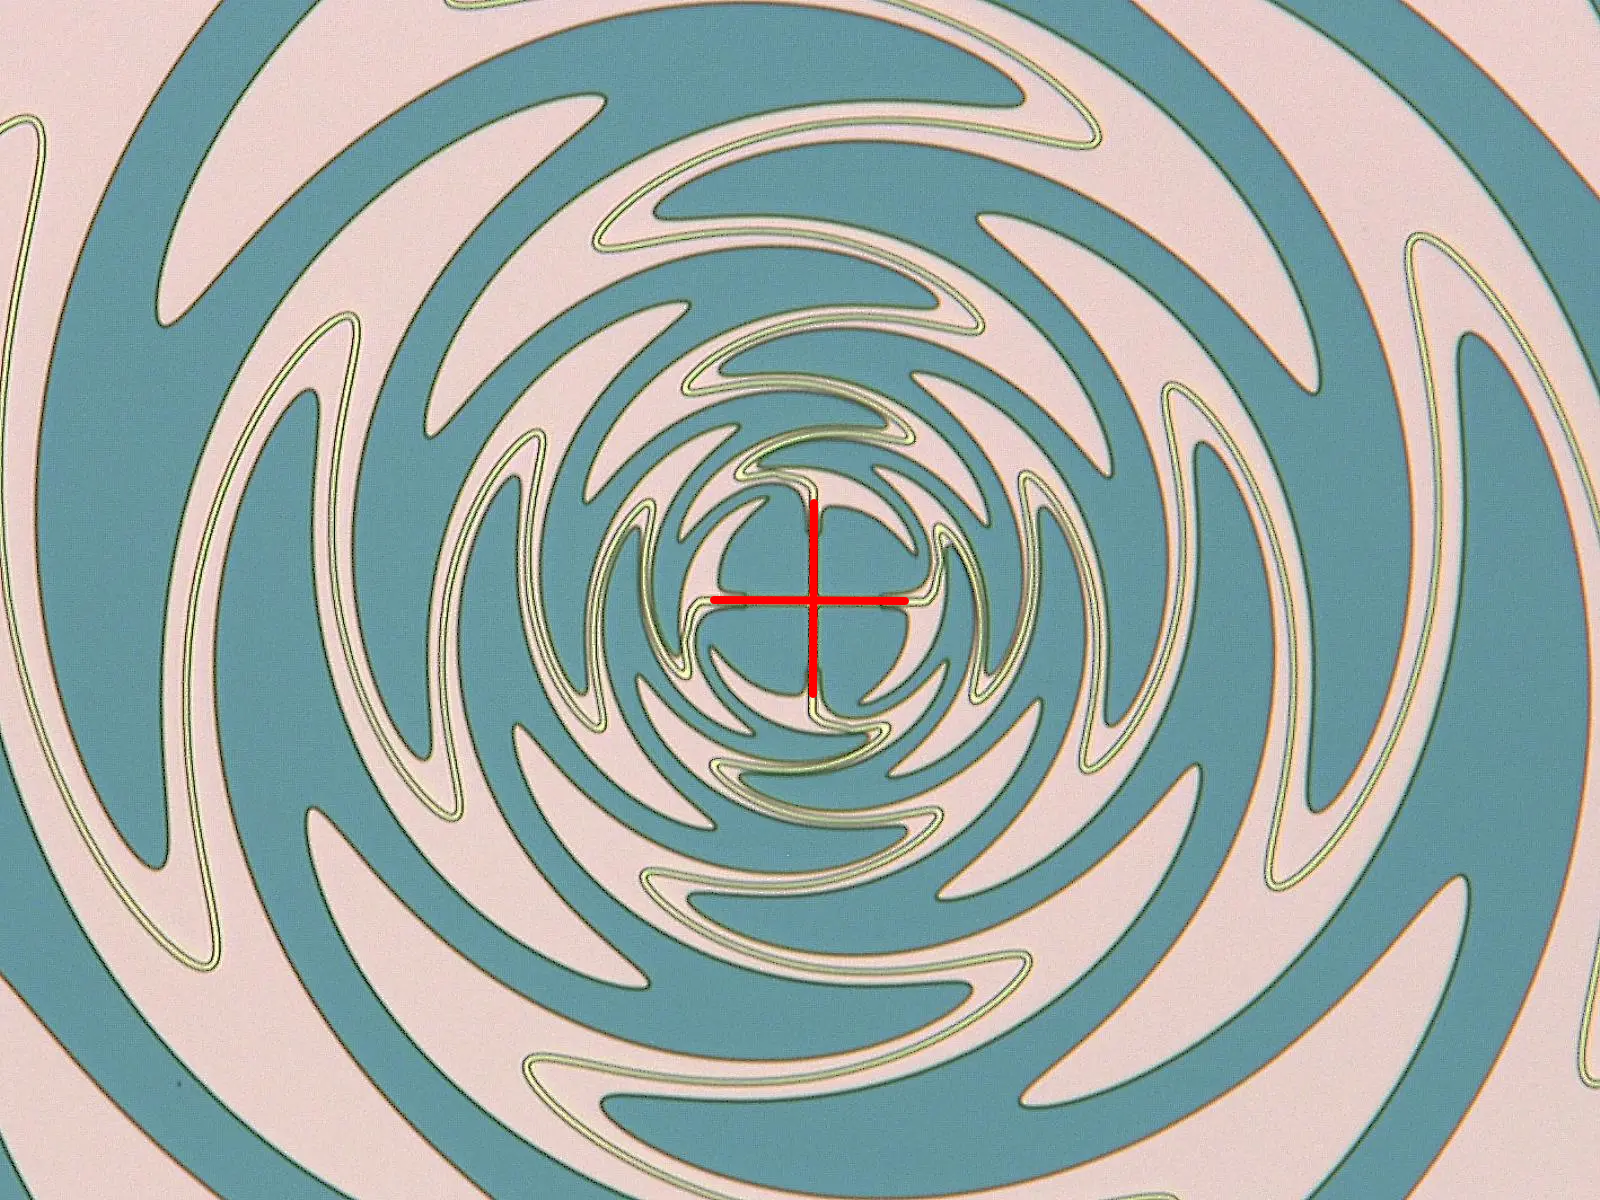
\includegraphics[width=\linewidth]{figures/sinuous-antenna-center-red.png}
        %   \caption{Center of a sinuous antenna detector used for Simons Observatory.}
        %   \label{fig:sinuous-antenna}
        % \end{wrapfigure}

        We assume that the atmospheric signal and the ground pickup are \emph{unpolarized}.
        The idea is to use the dual-polarization detectors
        %(see Figure~\ref{fig:sinuous-antenna}) 
        to eliminate non polarized signals:
        \[
          d_{A/B} = I \pm P
          \quad\longrightarrow\quad
          d_- = \frac12 \pab{d_A - d_B} = P
        \]

        This subtraction ideally decouples intensity and polarization components so that we can reconstruct the polarization signal \emph{exclusively} from the differenced TOD.
        This simple approach has been (and still is) used in CMB experiments such as Polarbear~\cite{Poletti:2016xhi} and BICEP/Keck~\cite{BICEP2:2014dgt}. % TODO: citations

        \heading{Advantages}

        \begin{itemize}
          \item Remove (most of) the unpolarized signals without any further assumptions or atmosphere models.
          \item Numerical benefits: atmosphere introduces long noise correlations, which worsen the \emph{conditioning} of the map-making system; removing those greatly speeds up the convergence (see Figure~\ref{fig:convergence}).
          \item Polarization maps reconstructed from the differenced TOD are formally equivalent to the GLS solution if we assume no particular model for the atmosphere (i.e. only that it is unpolarized and common to the orthogonal detectors in a pair).
        \end{itemize}

        \heading{Pitfalls}

        For the intensity signal to fully cancel, the two orthogonal detectors have to be \emph{identical}.
        Even with careful calibration, this can never be achieved perfectly.
        Because the contaminants are much brighter than the CMB polarization, this is a real problem for pair differencing.
        The most important effects which are expected to cause leakage of the intensity signal into the differenced TOD are:

        \begin{itemize}
          \item miscalibration of the detector gains
          \item bandpass differences
          \item different beam shapes
        \end{itemize}

        We would like to assess the impact of those effects and find out in what conditions pair differencing is a viable approach for producing maps of the CMB polarization for B-mode search.

      \end{alertblock}

    \end{column}

    \separatorcolumn

    \begin{column}{\colwidth}

      \begin{figure}
        \centering
        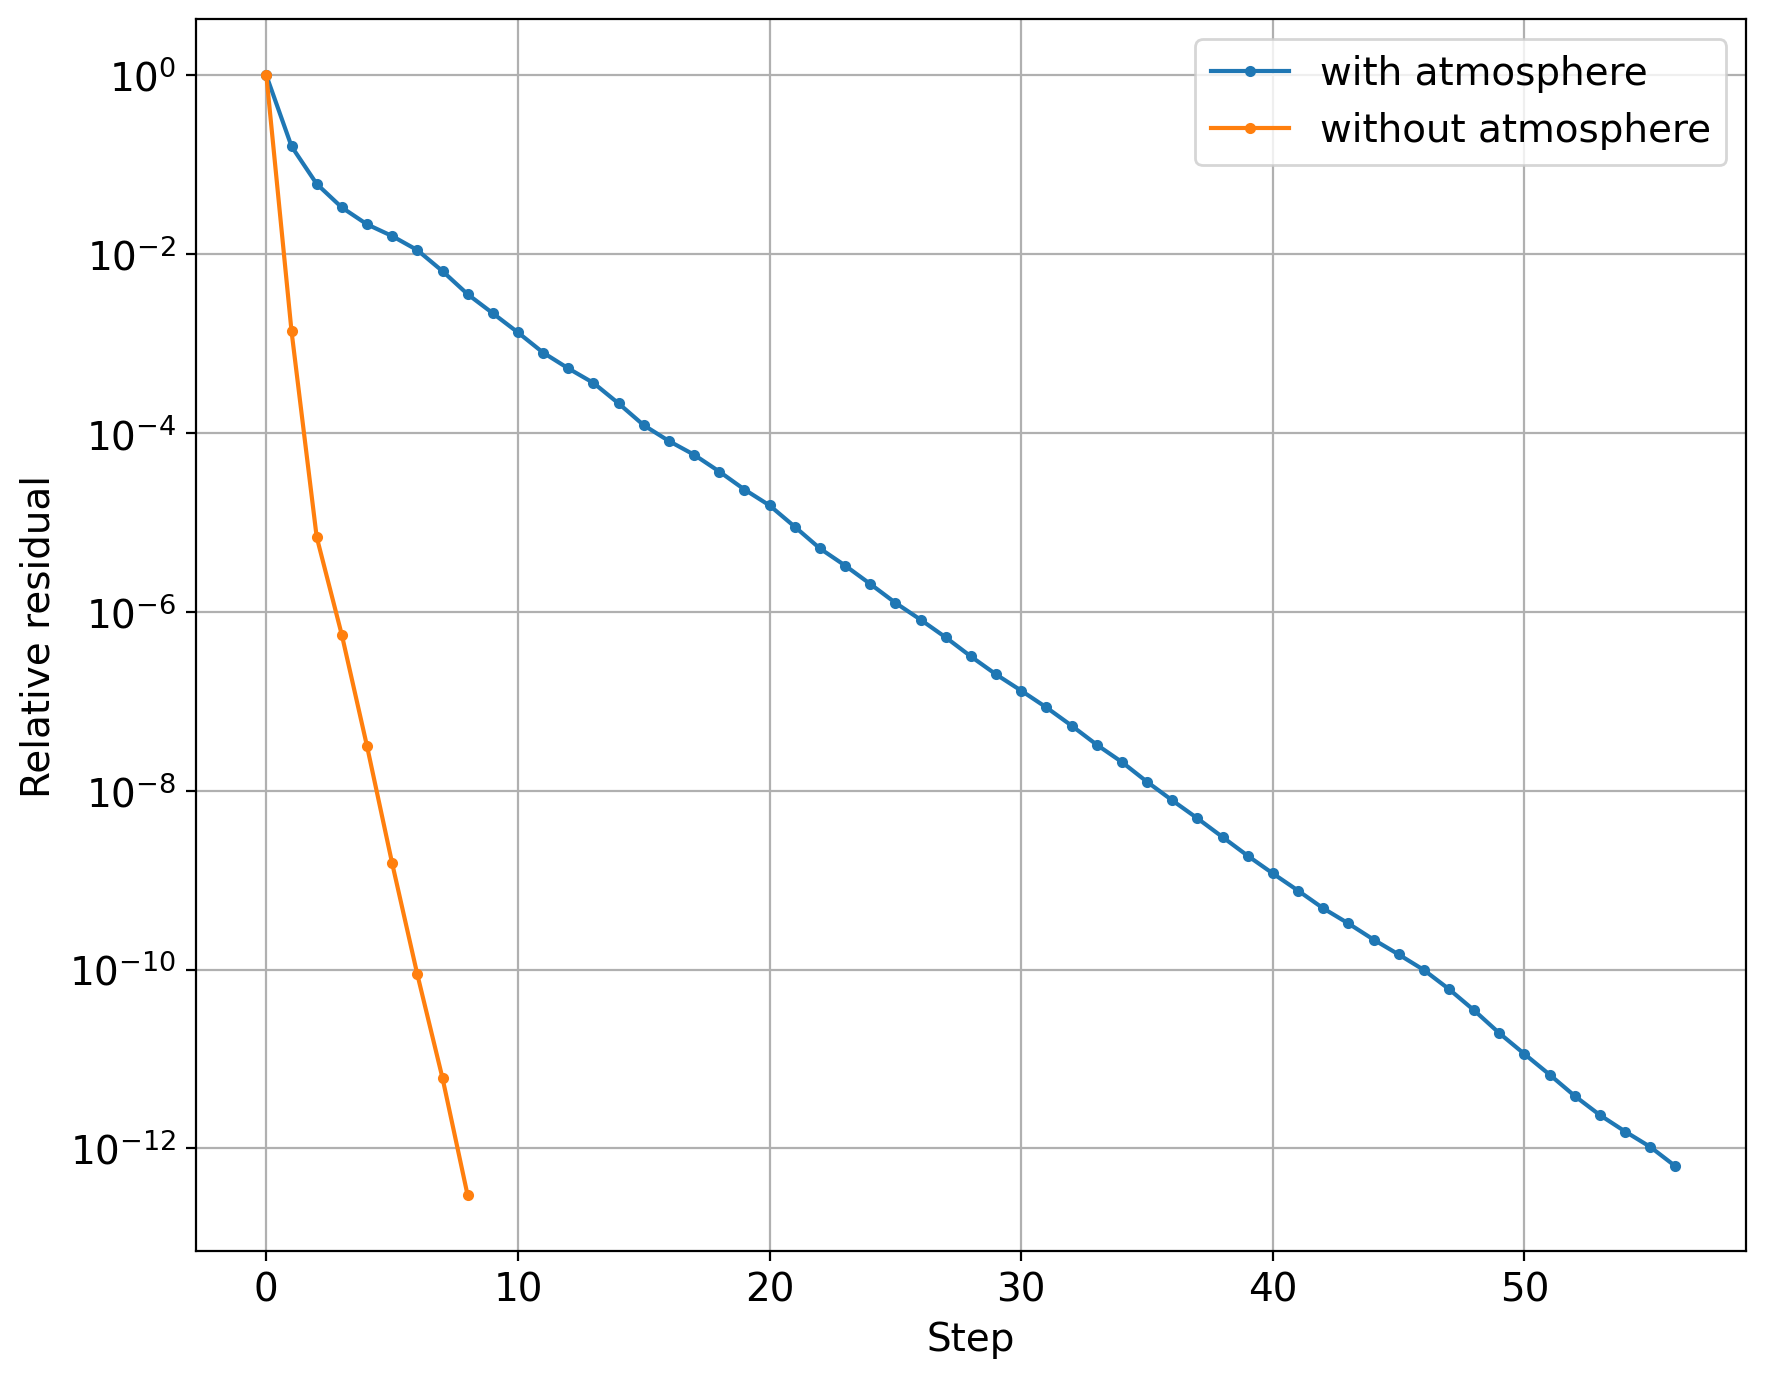
\includegraphics[width=0.8\textwidth]{figures/convergence.png}
        \caption{Convergence comparison with and without atmospheric correlations.}
        \label{fig:convergence}
      \end{figure}

      \begin{block}{Preliminary results}

        % The Simons Observatory (SO) is a ground-based CMB experiment located on Cerro Toco, $\qty[mode=text]{5200}{\meter}$ above sea level, in the Atacama desert of Chile.
        % The \say{nominal} SO experiment consists of three $\qty[mode=text]{0.4}{\meter}$ Small Aperture Telescopes (SATs) and one $\qty[mode=text]{6}{\meter}$ Large Aperture Telescope (LAT).

        Our current setup uses the TOAST framework for simulating data and the MAPPRAISER library~\cite{ElBouhargani:2021umq} for producing the sky maps.

        \begin{itemize}
          \item instrument: Simons Observatory Small Aperture Telescope @ $\qty[mode=text]{90}{\giga\hertz}$
          \item schedule: one day per month during one year
          \item sky: CMB lensed scalar anisotropies (from Planck FFP10 simulations)
          \item high-resolution atmosphere simulation
          \item instrumental noise
          \item gain errors of one percent in detector pairs
        \end{itemize}

        For the moment, we simply compare the B-mode residual spectra to the theoretical predictions.

        \begin{figure}
          \centering
          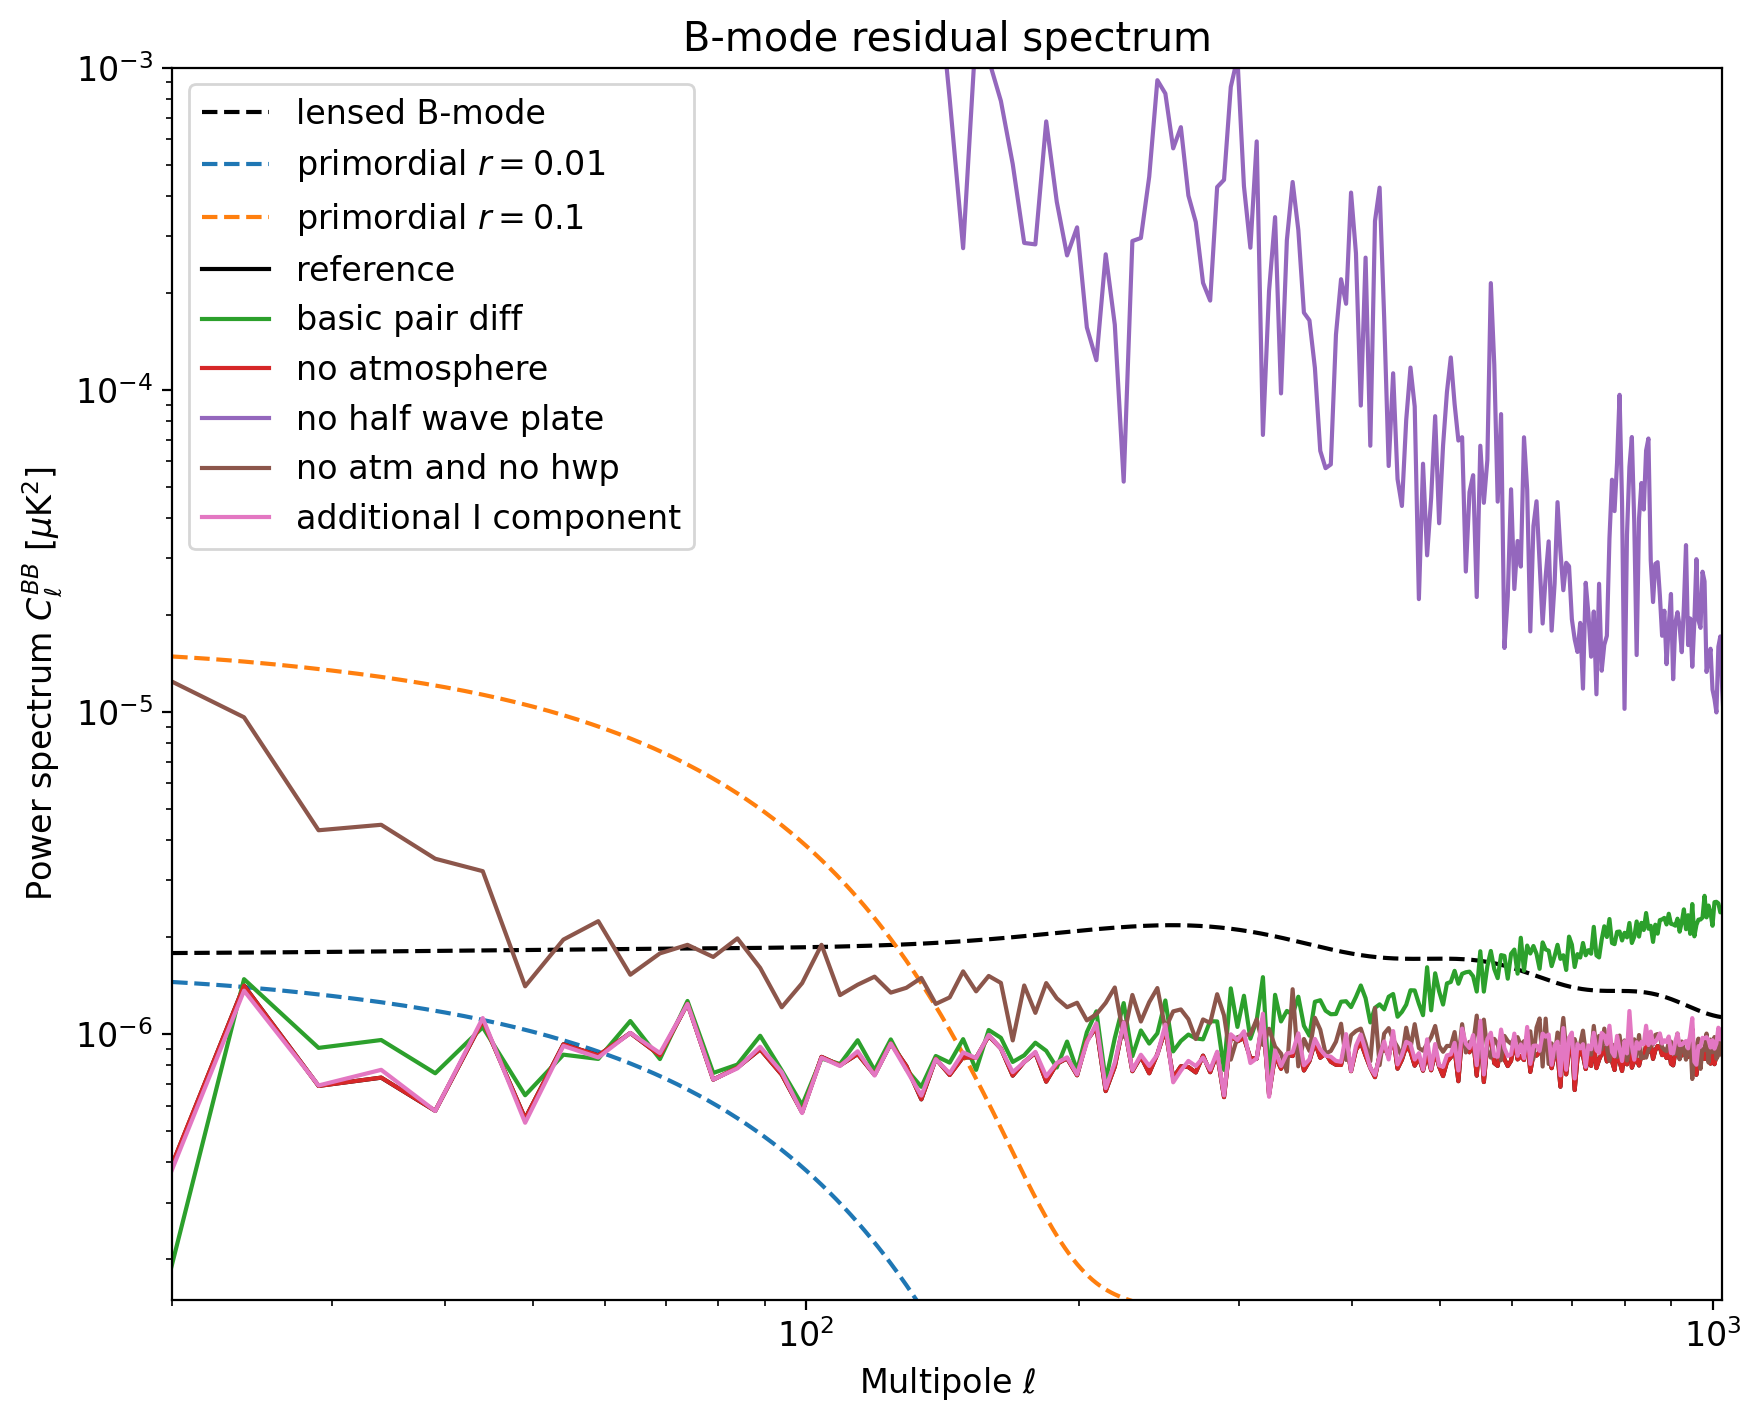
\includegraphics[width=0.8\textwidth]{figures/comparison.png}
          \caption{Resulting B-mode residual spectra for different configurations. Dashed lines represent theory BB spectra for $r$ equal to $\numlist[mode=text]{0;1e-3;1e-2}$. Solid lines are residual (noise) spectra.}
        \end{figure}

        Few comments on the figure?

      \end{block}

      \begin{block}{Future work, improvements}

        \begin{itemize}
          \item Refine simulations by adding bandpass and beam differences.
          \item Include realistic gain calibration error distributions.
          \item Perform a likelihood analysis to estimate biases and sensitivities to the tensor-to-scalar ratio.
        \end{itemize}

      \end{block}

      \begin{block}{References}

        \nocite{*}
        \footnotesize{\printbibliography}

      \end{block}

    \end{column}

    \separatorcolumn
  \end{columns}
\end{frame}

\end{document}
